\section{Architettura di sistema}
\subsection{\textit{Data processing architectures}}
Le architetture di tipo \textit{data processing} sono progettate per gestire l'\textit{ingestion}, \textit{processing} e memorizzazione di grandi quantità di dati.
Esse permettono di analizzare e ottenere informazioni utili (\textit{insight}) da questi dati, consentendo di ottimizzare i processi decisionali e migliorare le prestazioni aziendali.
Esistono diverse architettura, ciascuna con le proprie caratteristiche e vantaggi. Tra le più comuni troviamo l'architettura \textit{lambda} e l'architettura \textit{kappa}.

\subsubsection{Architettura \textit{lambda}}
L'architettura \textit{lambda} è costituita dalle seguenti quattro componenti:
\begin{itemize}
	\item \textbf{sorgente di dati}: responsabile dell'acquisizione dei dati grezzi da diverse sorgenti;
	\item \textbf{\textit{batch layer}}: responsabile dell'elaborazione e persistenza di dati storici in \textit{batch} di grandi dimensioni; il suo scopo è fornire risposte complete e accurate, anche se con una latenza più elevata rispetto allo \textit{speed layer}. Tale componente è tipicamente rappresentata da \textit{framework} come Apache Hadoop o Apache Spark;
	\item \textbf{\textit{speed (real-time) layer}}: responsabile dell'elaborazione e persistenza di dati in tempo reale. I dati vengono elaborati in modo rapido e con una latenza molto bassa, fornendo tuttavia risposte elaborate rispetto al \textit{batch layer}. Questa componente è tipicamente rappresentata da \textit{framework} come Apache Storm o Apache Flink;
	\item \textbf{\textit{serving layer}}: responsabile della fornitura dei dati elaborati in modo veloce ed affidabile, indipendentemente dal \textit{layer} di elaborazione utilizzato.
\end{itemize}

\begin{center}
	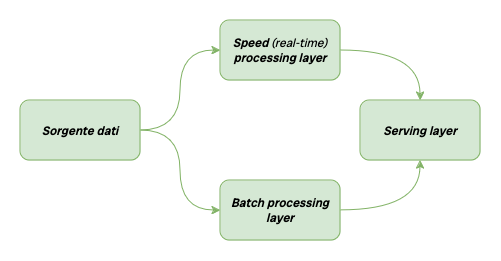
\includegraphics[width=0.6\textwidth]{./specifica_tecnica/architettura_lambda.png}
	\captionof{figure}{Architettura \textit{lambda}}
\end{center}

\subsubsubsection{Vantaggi e svantaggi}
L'architettura \textit{lambda} offre diversi vantaggi, tra cui la \textbf{scalabilità orizzontale}, la \textbf{tolleranza ai guasti} e la \textbf{flessibilità}. Tuttavia, la presenza
di due \textit{layer} di elaborazione separati può portare a problemi di coerenza dei dati, duplicazione della logica di aggregazione e complessità aggiuntiva nella gestione del sistema.
Inoltre, rispetto all'architettura \textit{kappa}, l'architettura \textit{lambda} può avere una latenza più elevata.

\subsubsubsection{Casi d'uso}
L'architettura \textit{lambda} è particolarmente adatta per applicazioni che richiedono sia un'analisi sui dati in tempo reale che un'analisi storica.

\subsubsection{Architettura \textit{kappa}}
L'architettura \textit{kappa} è stata introdotta per semplificare l'architettura \textit{lambda}, eliminando la necessità di gestire due \textit{layer} di elaborazione separati per il \textit{batch processing} e il \textit{real-time processing}.
Essa si divide in tre componenti principali:
\begin{itemize}
	\item \textbf{sorgente di dati}: responsabile dell'acquisizione dei dati grezzi da diverse sorgenti;
	\item \textbf{\textit{processing layer}}: responsabile dell'elaborazione dei dati in tempo reale, senza la necessità di separare i dati in \textit{batch} e \textit{real-time};
	\item \textbf{\textit{serving layer}}: responsabile della fornitura dei dati elaborati in modo veloce ed affidabile.
\end{itemize}

\begin{center}
	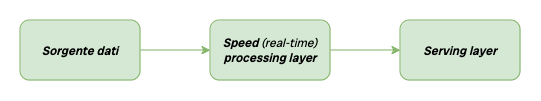
\includegraphics[width=0.6\textwidth]{./specifica_tecnica/architettura_kappa.png}
	\captionof{figure}{Architettura \textit{kappa}}
\end{center}

\subsubsubsection{Vantaggi e svantaggi}
L'architettura \textit{kappa} offre diversi vantaggi, tra cui la \textbf{semplicità}, la \textbf{riduzione dei costi} e la \textbf{bassa latenza}.
Tuttavia, può non essere adatta per applicazioni che richiedono un'analisi storica dei dati.

\subsubsubsection{Casi d'uso}
L'architettura \textit{kappa} è particolarmente adatta per gli scenari in cui sono critici i dati in tempo reale e l'analisi dei dati storici è meno importante. Inoltre, semplifica notevolmente il processo di sviluppo e manutenzione dei sistemi di elaborazione dei dati.

\subsection{Architettura scelta}
Nello scenario del capitolato proposto da \textit{SyncLab S.r.L.}, è critica l'analisi in tempo reale, in quanto i dati provenienti dai sensori IoT devono fornire informazioni sempre aggiornate ed eventualmente
sollevare allarmi in caso di situazioni critiche. Inoltre, non è richiesta l'aggregazione storica di dati, dunque i vantaggi dell'architettura \textit{lambda} non risultano utili per i nostri fini.
Per soddisfare tali requisiti, è stata dunque scelta l'architettura \textit{kappa}.

\subsubsection{Componenti di sistema}
All'interno del sistema da noi progettato sono dunque presenti le seguenti componenti:
\begin{itemize}
	\item \textbf{sorgenti di dati}: costituite dal simulatore di sensori, il quale genera i dati grezzi che in un contesto reale sarebbero provenienti dai sensori IoT;
	\item \textbf{\textit{streaming layer}}: gestisce il flusso di dati in tempo reale provenienti dai sensori. È composto da \textit{Redpanda} e lo \textit{Schema Registry};
	\item \textbf{\textit{processing layer}}: elabora i dati in tempo reale per calcolare metriche e indici. È composto da \textit{Apache Flink};
	\item \textbf{\textit{storage layer}}: memorizza i dati elaborati per l'analisi e la visualizzazione. È composto da \textit{ClickHouse};
	\item \textbf{\textit{data visualization layer}}: fornisce un'interfaccia utente per visualizzare i dati elaborati. È composto da \textit{Grafana}.
\end{itemize}

\begin{center}
	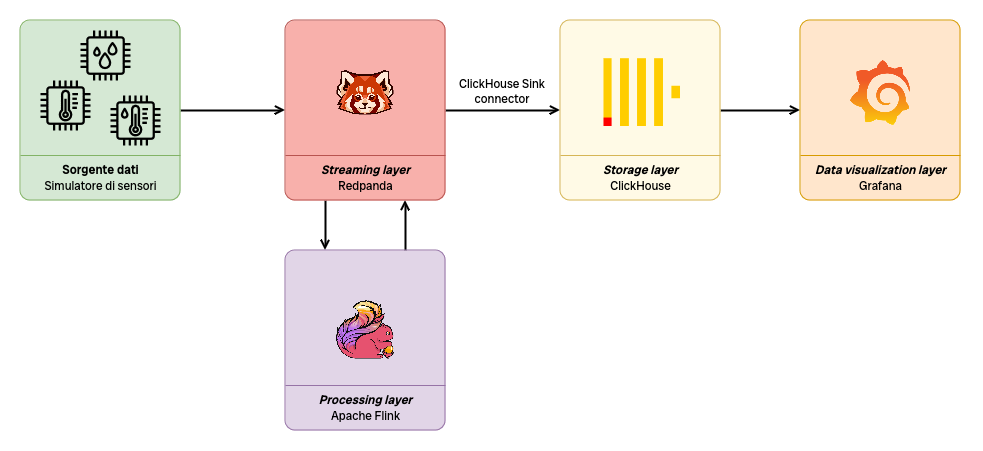
\includegraphics[width=0.7\textwidth]{./specifica_tecnica/architettura_sistema.png}
	\captionof{figure}{Componenti di sistema ad alto livello}
\end{center}

\subsubsection{Flusso di dati}
Per illustrare il flusso di dati all'interno del sistema, è stato realizzato il seguente diagramma, il quale mostra il percorso che i dati grezzi seguono dal simulatore fino alla visualizzazione tramite Grafana.
\begin{center}
	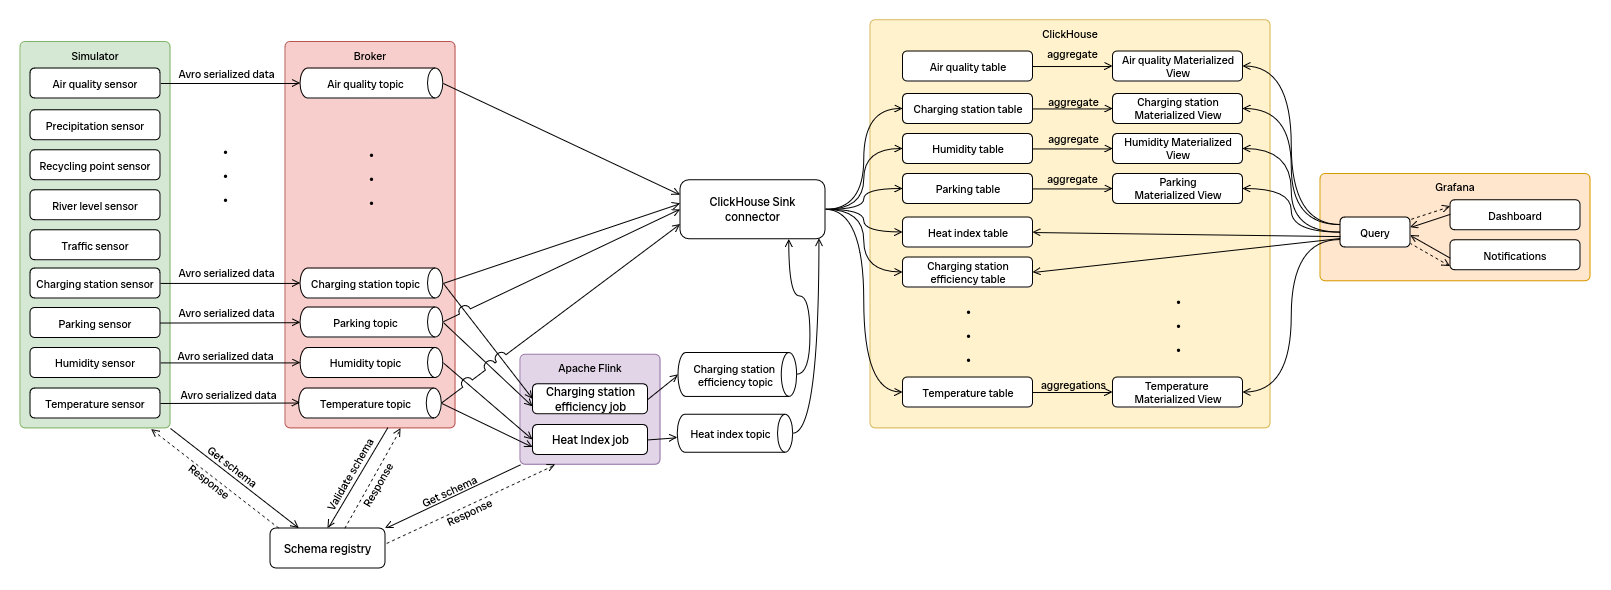
\includegraphics[width=1\textwidth]{./specifica_tecnica/data_flow.png}
	\captionof{figure}{Flusso di dati all'interno del sistema. I sensori di precipitazioni, isole ecologiche, livello dei fiumi e traffico sono stati omessi per chiarezza, ma il percorso di tali dati è analogo a quello dei sensori di qualità dell'aria.}
\end{center}
\linebreak
Il flusso seguito dai dati si può riassumere nei seguenti passaggi:
\begin{enumerate}
	\item \textbf{generazione dei dati}: ciascun simulatore emula il comportamento di un singolo sensore IoT, generando ad intervalli periodici o ad eventi (\textit{event-driven}) i dati grezzi relativi alla propria tipologia di dato.
	\item \textbf{serializzazione e produzione dei dati}: i dati grezzi generati nel punto precedente vengono serializzati utilizzando il formato Confluent Avro e inviati nel \textit{topic} corrispondente al tipo di dato generato;
	\item \textbf{elaborazione dei dati}: i \textit{topic} contenenti i dati grezzi di temperatura, umidità, occupazione dei parcheggi e colonnine di ricarica vengono consumati da Apache Flink.
	      Due \textit{job} distinti si occupano di calcolare la temperatura percepita e il grado di efficienza delle colonnine di ricarica. Una volta elaborati, i dati vengono inviati rispettivamente
	      nei \textit{topic} \texttt{heat\_index} e \texttt{charging\_station\_efficiency};
	\item \textbf{memorizzazione dei dati}: attraverso il connettore \textit{sink} per ClickHouse, i dati pubblicati in tutti i \textit{topic} vengono memorizzati nel database;
	\item \textbf{aggregazioni con \textit{materialized view}}: attraverso l'utilizzo di \textit{materialized view} in ClickHouse, vengono calcolate le statistiche relative ai dati memorizzati, come ad esempio la media oraria o giornaliera.
	      Tali aggregazioni sono più semplici rispetto a quelle effettuate da Flink, in quanto non richiedono elaborazioni complesse sui dati;
	\item \textbf{visualizzazione dei dati}: i dati memorizzati in ClickHouse vengono visualizzati tramite Grafana, che permette di creare \textit{dashboard} personalizzate per monitorare i dati in tempo reale;
	\item \textbf{notifiche}: Grafana esegue periodicamente delle \textit{query} per verificare se sono state superate delle soglie predeterminate. In caso affermativo, vengono inviate notifiche tramite il canale Discord dedicato, in modo tale da poter avvisare l'autorità locale.
\end{enumerate}

\subsection{Architettura dei simulatori}
I simulatori vengono utilizzati per produrre dati grezzi che sostituiscono le rilevazioni effettuate dai sensori IoT in un contesto reale.
Per tale motivo, questa parte del sistema non è ufficialmente parte del prodotto finale, ma è stata sviluppata per scopi di \textit{test}
e dimostrativi nell'ambito del progetto didattico; ai fini di quest'ultimo, il gruppo ha deciso di dedicare alcune risorse per la progettazione.\\
Nei paragrafi successivi verranno descritti i moduli che compongono i simulatori, le classi e metodi principali e i \textit{design pattern} utilizzati.\\
Sono stati implementati simulatori per i seguenti tipi dato:
\begin{itemize}
	\item qualità dell'aria;
	\item precipitazioni;
	\item isole ecologiche;
	\item livello dei fiumi;
	\item traffico;
	\item colonnine di ricarica;
	\item parcheggi;
	\item temperatura;
	\item umidità.
\end{itemize}

%TODO per ogni modulo bisogna:
% 1. Mettere foto diagramma delle classi UML
% 2. Descrizione ad alto livello di quello che fa il modulo
% 3. Descrivere i design pattern utilizzati
% 4. Descrivere le classi del modulo
%TODO diagramma progettazione sensori UML

\subsubsection{Modulo \texttt{models}}
Questo modulo contiene le classi che rappresentano i dati grezzi generati dai sensori (\texttt{raw\_data}) e la configurazione dei sensori stessi (\texttt{config}) letta
dal file di configurazione \texttt{sensors.toml} e dalle variabili d'ambiente.\\
Ciascun tipo di dato grezzo è rappresentato da una classe che estende la classe astratta \texttt{RawData}, la quale contiene i campi comuni a tutti i tipi di dato,
i metodi \textit{helper} \texttt{topic} e \texttt{value\_subject()} e il metodo \texttt{to\_json()} per la serializzazione in formato JSON.\\
Lo classe \texttt{SensorConfig} riceve nel costruttore la configurazione sotto forma di dizionario, effettua \textit{parsing}, validazione,
popola con valori di \textit{default} i campi mancanti (nel caso lo prevedano) ed inizializza i propri attributi, corrispondenti ai campi del file di configurazione.\\
Allo stesso modo, \texttt{EnvConfig} legge le variabili d'ambiente ed espone il metodo \texttt{bootstrap\_server()} che combina \textit{host} e \textit{port} per formare l'indirizzo del \textit{broker} Kafka.\\

\begin{center}
	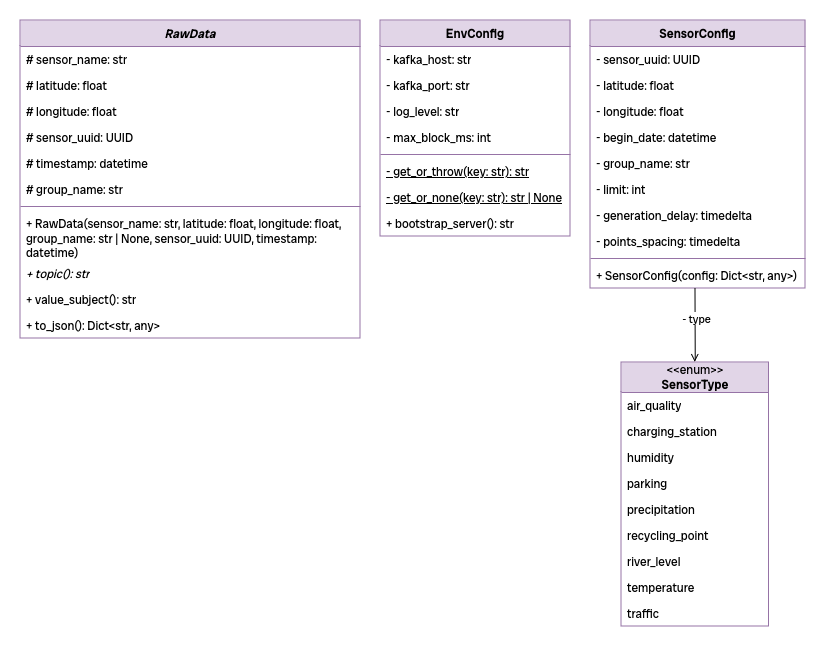
\includegraphics[width=0.87\textwidth]{./specifica_tecnica/models.png}
	\captionof{figure}{Diagramma delle classi del modulo \texttt{models}}
\end{center}


\subsubsection{Modulo \texttt{producers}}
\begin{center}
	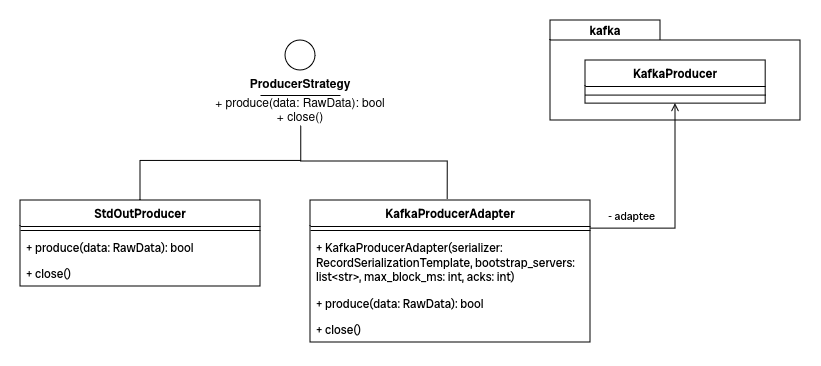
\includegraphics[width=0.87\textwidth]{./specifica_tecnica/producers.png}
	\captionof{figure}{Diagramma delle classi del modulo \texttt{producers}}
\end{center}

\subsubsection{Modulo \texttt{serializers}}
\begin{center}
	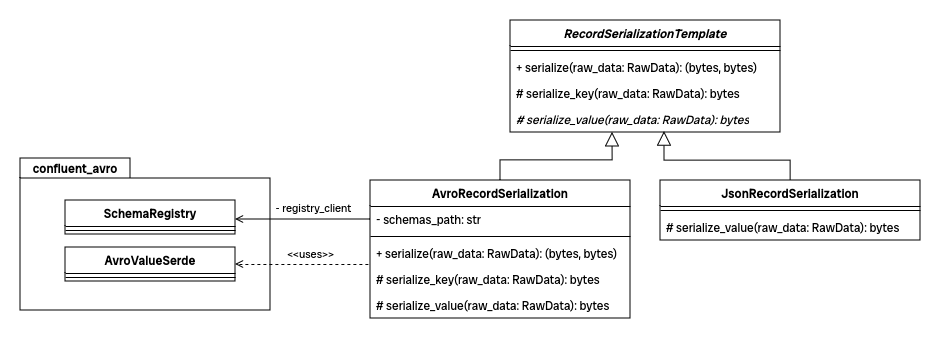
\includegraphics[width=0.87\textwidth]{./specifica_tecnica/serializers.png}
	\captionof{figure}{Diagramma delle classi del modulo \texttt{serializers}}
\end{center}

\subsubsection{Modulo \texttt{simulators}}
% TDOD diagramma simulators

\subsection{Redpanda}
\subsubsection{Kafka topic}
I Kafka topic sono categorie o canali di messaggi all'interno di \textit{Redpanda}. Un topic in Kafka è come una cassetta postale virtuale o una categoria di messaggi in cui i dati vengono pubblicati dai produttori e letti dai consumatori.

\subsubsubsection{Formato dei dati e Schema Registry}
% Ciascun tipo di dato viene inviato su un topic specifico, in modo da poter essere elaborato in modo indipendente.
% TODO: parlare di Confluent Avro, del formato di serializzazione delle chiavi e partitioning strategy e di topic name strategy <topic>-value

\subsection{Flink - \textit{Processing layer}}
\subsubsection{Introduzione}
È un \textit{framework} di elaborazione dati distribuito e \textit{open-source} che si distingue per la sua capacità di gestire sia dati di flusso in tempo reale che dati \textit{batch}.
Una delle sue caratteristiche principali è la capacità di gestire dati in tempo reale con latenze molto basse.
Ciò significa che può elaborare i dati man mano che arrivano, consentendo alle applicazioni di reagire istantaneamente ai cambiamenti nell'\textit{input}.
Questa caratteristica è particolarmente importante per le applicazioni che richiedono analisi in tempo reale, come il monitoraggio di sensori, il rilevamento di
anomalie o la personalizzazione di contenuti.

\subsubsection{Componenti Flink e \textit{processing layer}}
È costituito da diverse componenti fondamentali che lavorano insieme per consentire l'elaborazione efficiente e scalabile dei dati in tempo reale e batch. Queste componenti formano il cuore del sistema Flink e forniscono le basi per la sua potente capacità di elaborazione dei dati.
% In questa sezione, esamineremo le principali componenti di Flink e il loro ruolo nella creazione di un'infrastruttura robusta per l'analisi dei dati.
% \begin{itemize}
% 	\item \textbf{JobManager}: è il componente centrale di Flink responsabile della pianificazione e del coordinamento dei job di elaborazione dei dati. Gestisce il flusso di lavoro complessivo, assegnando i task ai TaskManager per l'esecuzione;
% 	\item \textbf{TaskManager}: è responsabile dell'esecuzione effettiva delle operazioni di elaborazione dei dati, eseguendo i task assegnati loro dal JobManager e gestendo il caricamento, l'elaborazione e la distribuzione dei dati all'interno del cluster;
% 	\item \textbf{\textit{Processing layer}}: è responsabile dell'esecuzione delle operazioni di elaborazione dei dati all'interno del cluster distribuito. Questa layer sfrutta le risorse di calcolo e memorizzazione disponibili nei nodi del cluster per eseguire le operazioni di trasformazione, aggregazione, filtraggio e altro ancora sui dati in ingresso. Utilizzando un modello di esecuzione distribuita, la \textit{Processing layer} di Flink è in grado di scalare orizzontalmente per gestire grandi volumi di dati e carichi di lavoro ad alta intensità computazionale.
% \end{itemize}
\subsubsection{\textit{Processing layer data-flow}}
%TODO mettere foto del processing layer data-flow di flink
% \begin{enumerate}
% 	\item \textbf{Acquisizione dei dati};
% 	\item \textbf{partizione e distribuzione}: i dati vengono divisi in parti più piccole e distribuiti tra i nodi del cluster per massimizzare l'utilizzo delle risorse;
% 	\item \textbf{pianificazione dei task}: il JobManager assegna compiti di elaborazione ai TaskManager basandosi sullo stato del cluster e sull'ottimizzazione delle prestazioni;
% 	\item \textbf{esecuzione dei task}: i TaskManager eseguono i compiti assegnati in parallelo, elaborando i dati in base alla logica definita nell'applicazione Flink;
% 	\item \textbf{scambio e movimento dei dati}: i dati possono essere scambiati e spostati tra i nodi del cluster per supportare operazioni complesse come il join o l'aggregazione;
% 	\item \textbf{persistenza e output}: una volta elaborati, i risultati vengono eventualmente salvati o inviati ad altre destinazioni per l'analisi o l'utilizzo successivo.
% \end{enumerate}

\subsubsection{\textit{Job}}
\subsubsubsection{\textit{Heat Index}}
A partire dai dati rilevati dai sensori di temperatura e umidità; esso consente di stimare la percezione della temperatura da parte dell'essere umano.
Nella configurazione del Simulatore, oltre a posizione e identificativo per ciascun sensore, è possibile specificare un \texttt{group\_name}, una stringa che identifica il gruppo o zona di appartenenza;
si suppone che sensori situati in posizioni geografiche vicine abbiano lo stesso \texttt{group\_name}. Il \textit{job} calcola prima separatamente
la temperatura e l'umidità media per finestre di un'ora, aggregando i dati provenienti da sensori dello stesso gruppo. Successivamente con i valori ottenuti computa lo \textit{Heat Index},
utilizzando la \underline{\href{https://www.ncbi.nlm.nih.gov/pmc/articles/PMC3801457/}{formula empirica ideata da Blazejczyk}} [Ultima consultazione 2024-06-25].
Nel risultato finale, oltre al valore dello \textit{Heat Index}, vengono restituiti anche i valori di temperatura e umidità medi, il centro di massa del gruppo di sensori
(utilizzando la formula \underline{\href{https://en.wikipedia.org/wiki/Haversine_formula}{Haversine}} [Ultima consultazione 2024-06-25] per il calcolo della distanza) e la
distanza dal centro di massa al sensore più lontano. Questi ultimi due dati sono impiegati in una mappa interattiva su Grafana per poter disegnare un cerchio, rappresentante la zona di influenza del gruppo di sensori.
\subsubsubsection{Efficienza delle colonnine elettriche}
% TODO: aggiungere dettagli implementativi

% KPI che useremo :european air quality index, heat index, charging station efficiency index


\subsection{Database ClickHouse}
% Come detto in precedenza, il database adottato è \textit{ClickHouse}. Per ogni sensore è stata creata una tabella \textit{MergeTree}, che permette di memorizzare i dati in modo efficiente e di eseguire query complesse in modo veloce.

\subsubsection{Funzionalità utilizzate}
\subsubsubsection{Materialized View}
Sono una potente funzionalità di \textit{ClickHouse} per migliorare le prestazioni delle query e semplificare l'analisi dei dati. In sostanza, una materialized view è una vista pre-calcolata o una copia di una query, memorizzata fisicamente su disco in forma tabellare. Ciò consente di evitare il calcolo ripetuto dei risultati della query ogni volta che viene eseguita.
\subsubsubsection*{Documentazione}
\url{https://clickhouse.com/docs/en/guides/developer/cascading-materialized-views}

[Ultima consultazione 2024-06-05]

\subsubsubsection*{Utilizzi}
% TODO: utilizzi nel progetto
% \begin{itemize}
% 	\item \textbf{Aggregazioni pre-calcolate}: le materialized view possono essere utilizzate per memorizzare i risultati di aggregazioni complesse, come somme, medie, conteggi, ecc., in modo che non debbano essere calcolati ogni volta che viene eseguita una query;
% 	\item \textbf{rapporti pre-calcolati}: possono essere utilizzate per memorizzare i risultati di query complesse o di rapporti, in modo che i risultati siano immediatamente disponibili senza dover eseguire la query ogni volta;
% 	\item \textbf{join ottimizzati}: possono essere utilizzate per memorizzare i risultati di join complessi tra più tabelle, in modo che i risultati siano immediatamente disponibili senza dover eseguire il join ogni volta;
% 	\item \textbf{filtraggio e selezione efficiente}: possono essere utilizzate per filtrare e selezionare dati in base a criteri specifici, migliorando le prestazioni delle query che richiedono l'accesso solo a una parte dei dati.
% 	\item \textbf{Analisi dei dati storici}: i dati storici vengono memorizzati in tabelle MergeTree per consentire l'analisi e l'elaborazione dei dati storici;
% 	\item \textbf{applicazioni di business intelligence}: i dati vengono memorizzati in tabelle MergeTree per consentire l'analisi e la generazione di report per le applicazioni di business intelligence;
% 	\item \textbf{log e monitoraggio}: i dati di log e di monitoraggio vengono memorizzati in tabelle MergeTree per consentire l'analisi e il monitoraggio delle attività di sistema.
% \end{itemize}
\subsubsubsection{MergeTree}
MergeTree è uno dei principali motori di archiviazione di ClickHouse, progettato per gestire grandi volumi di dati e fornire elevate prestazioni di lettura e scrittura. È particolarmente adatto per applicazioni in cui i dati vengono aggiunti in modo incrementale e le query vengono eseguite su intervalli di tempo specifici.
Le caratteristiche principali sono:
\begin{itemize}
	\item \textbf{partizionamento}, in cui i dati vengono partizionati in base a una colonna di data o di tempo, in modo che i dati più recenti siano memorizzati in partizioni separate e possano essere facilmente eliminati o archiviati;
	\item \textbf{ordine dei dati}, dove i dati vengono ordinati in base a una colonna di ordinamento, in modo che i dati siano memorizzati in modo sequenziale e possano essere letti in modo efficiente;
	\item \textbf{indice primario}, tramite il quale i dati vengono indicizzati in base a una colonna di chiave primaria, in modo che le query di ricerca e di join siano veloci ed efficienti;
	\item \textbf{merging dei dati}, in questo modo i dati vengono uniti in modo incrementale in background, in modo che le query di aggregazione e di analisi siano veloci ed efficienti;
	\item \textbf{compressione}, i dati vengono compressi in modo efficiente per ridurre lo spazio di archiviazione e migliorare le prestazioni di lettura e scrittura;
	\item \textbf{replica e distribuzione}, i dati possono essere replicati e distribuiti su più nodi per garantire l'affidabilità e la disponibilità del sistema.
\end{itemize}
\subsubsubsection*{Documentazione}
\url{https://clickhouse.com/docs/en/engines/table-engines/mergetree-family/mergetree}

[Ultima consultazione 2024-06-05]

\subsubsection{Trasferimento dati tramite Materialized View}
Le Materialized View in ClickHouse sono viste che memorizzano fisicamente i risultati di una query specifica in modo da permettere un accesso rapido e efficiente ai dati pre-elaborati. Quando vengono create, le Materialized View eseguono la query definita e archiviano i risultati in una struttura di dati ottimizzata per l'accesso veloce. Questo consente di evitare il calcolo ripetuto dei risultati della query ogni volta che viene eseguita, migliorando notevolmente le prestazioni complessive del sistema. I vantaggi derivanti da questo approccio sono molteplici, tra questi troviamo:
\begin{itemize}
	\item \textbf{prestazioni ottimizzate}: grazie alla memorizzazione fisica dei risultati delle query, le Materialized View consentono un accesso rapido ai dati pre-elaborati, riducendo i tempi di risposta delle query complesse;
	\item \textbf{riduzione del carico di lavoro}: trasferendo i dati pre-elaborati in Materialized View, si riduce il carico di lavoro sul sistema sorgente, consentendo una maggiore scalabilità e riducendo il rischio di sovraccarico del sistema durante le operazioni di estrazione dei dati;
	\item \textbf{sempre aggiornate}: possono essere progettate per aggiornarsi automaticamente in risposta alle modifiche nei dati sottostanti, garantendo che i risultati siano sempre aggiornati e coerenti con lo stato attuale dei dati;
	\item \textbf{semplificazione dell'architettura}: è possibile semplificare l'architettura complessiva del sistema eliminando la necessità di eseguire query complesse e costose ogni volta che si accede ai dati.
\end{itemize}
%TODO prendere le query che creano le materialized view
\subsubsection{Misurazioni isole ecologiche}
Di seguito viene riportata la configurazione della tabella per le misurazioni delle isole ecologiche. Le misurazioni includono:
\begin{itemize}
	\item \textbf{sensor\_uuid}: identificativo univoco del sensore (formato UUID);
	\item \textbf{sensor\_name}: nome del sensore (formato String);
	\item \textbf{timestamp}: data e ora della misurazione (formato DateTime64);
	\item \textbf{latitude}: latitudine del sensore (formato Float64);
	\item \textbf{longitude}: longitudine del sensore (formato Float64);
	\item \textbf{filling\_value}: percentuale di riempimento dell'isola ecologica (formato Float32).
\end{itemize}
%TODO mettere foto della tabella isole ecologiche
\subsubsection{Misurazioni temperatura}
Di seguito viene riportata la configurazione della tabella per le misurazioni della temperatura. Le misurazioni includono:
\begin{itemize}
	\item \textbf{sensor\_uuid}: identificativo univoco del sensore (formato UUID);
	\item \textbf{sensor\_name}: nome del sensore (formato String);
	\item \textbf{timestamp}: data e ora della misurazione (formato DateTime64);
	\item \textbf{value}: valore della temperatura rilevata (formato Float32);
	\item \textbf{latitude}: latitudine del sensore (formato Float64);
	\item \textbf{longitude}: longitudine del sensore (formato Float64);
\end{itemize}
%TODO mettere foto della tabella temperatura
\subsubsection{Misurazioni traffico}
Di seguito viene riportata la configurazione della tabella per le misurazioni della traffico. Le misurazioni includono:
\begin{itemize}
	\item \textbf{sensor\_uuid}: identificativo univoco del sensore (formato UUID);
	\item \textbf{sensor\_name}: nome del sensore (formato String);
	\item \textbf{timestamp}: data e ora della misurazione (formato DateTime64);
	\item \textbf{latitude}: latitudine del sensore (formato Float64);
	\item \textbf{longitude}: longitudine del sensore (formato Float64);
	\item \textbf{vehicles}: numero di veicoli rilevati (formato Int32);
	\item \textbf{avg\_speed}: velocità media del traffico (formato Float32).
\end{itemize}
%TODO mettere foto della tabella traffico
\subsection{Grafana}
Grafana è uno strumento di analisi e monitoraggio che permette di visualizzare dati provenienti da una varietà di fonti. È sviluppato principalmente in Go e Typescript ed è noto per la sua capacità di creare dashboard personalizzabili e intuitive.
\subsubsection{Dashboard}
%metti stessa cosa del manuale utente riguardo le dashboard. 

\subsubsection{ClickHouse datasource plugin}
Il plugin ClickHouse per Grafana è un'implementazione che consente di utilizzare ClickHouse come fonte di dati per Grafana. Questo plugin facilita la connessione e l'interrogazione dei dati archiviati in ClickHouse direttamente da Grafana, permettendo di creare dashboard dinamiche e interattive.
\subsubsubsection*{Documentazione}
\url{https://grafana.com/grafana/plugins/grafana-clickhouse-datasource/}

[Ultima consultazione 2024-06-05]
\subsubsubsection{Configurazione del Datasource}
La configurazione  grafana/provisioning/datasources/default.yaml


\subsubsection{Variabili Grafana}
\subsubsubsection{Documentazione}
\url{https://grafana.com/docs/grafana/latest/dashboards/variables/}

[Ultima consultazione 2024-06-05]
\subsubsubsection*{Variabili nella dashboard principale}
Le variabili presenti nella dashboard principale sono:
\begin{itemize}
	\item \textbf{tipo sensore}: permette di selezionare il tipo di sensore da visualizzare (temperatura, traffico, isola ecologica...);
	\item \textbf{nome sensore}: permette di selezionare il nome del sensore da visualizzare (ad esempio sensore1, sensore2, ecc.); % TODO
\end{itemize}
%TODO mettere foto codice query
\subsubsubsection*{Variabili nella dashboard dettagliata}
Le variabili presenti nelle dashboard dettagliate sono:
\begin{itemize}
	\item \textbf{nome sensore}: permette di selezionare il nome del sensore da visualizzare (es. sensore1, sensore2, ecc.);
\end{itemize}

\subsubsection{Grafana Alerts}
Sono una funzionalità che permettono di definire, configurare e gestire avvisi basati su condizioni specifiche rilevate nei dati monitorati. Questi avvisi consentono agli utenti di essere informati tempestivamente su eventuali problemi o cambiamenti critici nei loro sistemi, applicazioni o infrastrutture.
\subsubsubsection*{Documentazione}
\url{https://grafana.com/docs/grafana/latest/alerting/} [Ultima consultazione 2024-06-05]
\subsubsubsection{Configurazione delle regole di alert}
Definiscono le condizioni che devono essere soddisfatte per attivare un alert. Gli eventi che generano un alert sono:
\begin{itemize}
	\item temperatura maggiore di 40°C per più di 30 minuti;
	\item isola ecologica piena al 100\% per più di 24 ore;
	\item superamento dell'indice 3 dell'EAQI (indice di qualità dell'aria);
	\item livello di precipitazioni superiore a 10 mm in 1 ora.
\end{itemize}
Gli alert possono possedere tre diversi tipi di stati:
\begin{itemize}
	\item \textbf{\textit{normal}}, indica che l'alert non è attivo perché le condizioni definite per l'attivazione dell'avviso non sono soddisfatte;
	\item \textbf{\textit{pending}}, indica che le metriche monitorate stanno iniziando a deviare dalle condizioni normali ma non hanno ancora soddisfatto completamente le condizioni per attivare l'alert;
	\item \textbf{\textit{firing}}, significa che le condizioni definite per l'avviso sono state soddisfatte e l'alert è attivo.
\end{itemize}
\subsubsubsection{Configurazione canale di notifica}
Per configurare un canale di notifica è necessario:
\begin{enumerate}
	\item nel menù di sinistra, cliccare sull'icona "Alerting";
	\item selezionare la voce "Notification channels";
	\item cliccare sul pulsante "Add channel" per aggiungere un nuovo canale di notifica;
	\item selezionare il tipo di canale di notifica desiderato tra quelli disponibili;
	\item configurare le impostazioni del canale di notifica in base alle proprie esigenze;
	\item cliccare sul pulsante "Save" per salvare le impostazioni del canale di notifica.
\end{enumerate}
% \textit{7Last} ha deciso di rendere risponibile il server \textit{Discord} configurato a questo scopo e raggiungibile a questo link:
% \begin{center}
% 	\url{https://discord.com/channels/1214553333113556992/1241974479345942568}
% \end{center}
\subsubsection{Altri plugin}
\subsubsubsection{Orchestra Cities Map plugin}
Progettato per facilitare la visualizzazione e l'analisi dei dati geospaziali all'interno di piattaforme di pianificazione urbana e sviluppo territoriale.\\
Le principali funzionalità offerte da questo plugin sono:
\begin{itemize}
	\item \textbf{visualizzazione dei dati geospaziali}: consente agli utenti di visualizzare dati geografici, come mappe, strati di dati GIS (Geographic Information System), punti di interesse e altre informazioni territoriali;
	\item \textbf{interfaccia interattiva}: offre un'interfaccia utente intuitiva e interattiva che consente agli utenti di esplorare e interagire con i dati geospaziali in modo dinamico;
	\item \textbf{personalizzazione}: offre opzioni di personalizzazione per adattarsi alle esigenze specifiche dell'utente o dell'applicazione;
	\item \textbf{analisi dei dati}: oltre alla semplice visualizzazione dei dati geospaziali, il plugin può anche supportare funzionalità avanzate di analisi dei dati, come l'identificazione di cluster, la creazione di heatmap e l'esecuzione di analisi spaziali per identificare tendenze o pattern significativi nei dati territoriali;
	\item \textbf{integrazione}: è progettato per integrarsi facilmente con altre componenti dell'ecosistema Orchestra Cities e con altre piattaforme software di pianificazione urbana e sviluppo territoriale.
\end{itemize}

\subsubsubsection*{Documentazione}
\url{https://grafana.com/grafana/plugins/orchestracities-map-panel/?tab=installation}

[Ultima consultazione 2024-06-05]
